\documentclass[12pt]{article}
%Gummi|065|=)
\usepackage{amsmath, amsfonts, amssymb}
\usepackage[margin=0.5in]{geometry}
\usepackage{xcolor}
%\usepackage{graphicx}
%\usepackage{graphicx}
\newcommand{\off}[1]{}
\DeclareMathSizes{20}{30}{21}{18}

\newcommand{\myhrule}{}

\newcommand{\two }{\sqrt[3]{2}}
\newcommand{\four}{\sqrt[3]{4}}

\newcommand{\dash}{
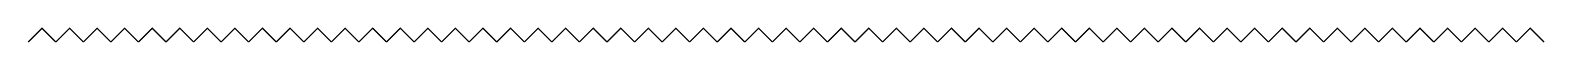
\begin{tikzpicture}[scale=0.35]
\foreach \x in {1,...,55}{
	\draw (\x,-0.25)--(\x+0.5,0.25)--(\x+1,-0.25);
}
\end{tikzpicture}
}

\newcommand{\sq}[3]{
\node at (#1+0.5,#2+0.5) {#3};
\draw (#1+0,#2+0)--(#1+1,#2+0)--(#1+1,#2+1)--(#1+0,#2+1)--cycle;
}

\usepackage{tikz}

\title{\textbf{ Examples: $n!$ the Factorial}}
\author{John D Mangual}
\date{}
\begin{document}

\fontfamily{qag}\selectfont \fontsize{25}{30}\selectfont

\maketitle

\noindent There are famous McMahon formulas and I could be mixing them up.  Here is one, which counts literally \textit{all} plane paritions:
$$ \sum_{\pi} q^{|\pi|} = \prod_{n=1}^\infty \left( \frac{1}{1-q^n} \right)^n$$
My apology in advance for not having a good picture.  They are take some work to draw.  Here we take example from Mirjana Vuletic.

\includegraphics{boxes.png} \\
This is good but not really what I am looking for today.

\newpage

\noindent I am looking for those partitions which fit inside an $a \times b \times c$ box.  There is an exact number on Wikipedia:
$$ \# \{ boxes\} = \prod_{i=1}^a 
\prod_{j=1}^b
\prod_{k=1}^c \frac{i+j+k-1}{i+j+k-2}$$
and you might wonder why so much attention might be drawn to a simple equation like this:
\begin{itemize}
\item Inside Mathematics - literally thousands of papers and they keep coming
\item Outside Mathematics - maybe a statistician or data analyst might find this structure relates to something in the real world\footnote{Baseball, elections, the human genome, the weather, instagram, the radio... and the end of the day these are all tables of numbers and there exist procedures where these can processed in a similar ways.}
\end{itemize}
Today we will do something totally useless and set $a = b = c = \frac{1}{2}$.  How many ways to pack $1 \times 1 \times 1$ cubes into a box of side $\frac{1}{2}\times \frac{1}{2} \times \frac{1}{2}$ ? \\ \\
The procedure for guessing a value of $(\frac{1}{2})!$ might stem from Euler's definition of factorial:
$$ x! = \lim_{n \to \infty} \frac{n^x \, n!}{x \times (x+1)\times (x+2)\times \dots (x+n)} $$

\newpage

\noindent Let's try to shift the product lattice by $(x,y,z)$:
$$  
\prod_{i=1}^a 
\prod_{j=1}^b
\prod_{k=1}^c \frac{(i+j+k)+(x+y+z)-1}{(i+j+k)+(x+y+z)-2} $$
I don't even know what this number is.  OK.  Let
$$ n!! = 0! \times 1! \times \dots \times (n-1)! $$
and we can even define the $q$-factorial 
$$[n]_q! := \prod_{i=1}^n \frac{1 -q^n}{1-q} $$
The hyperfactorial (and the Barnes G-function)
$$ \sum_\pi q^{|\pi|} = \frac{a!!_q b!!_q c!!_q (a+b+c)!!_q}{(a+b)!!_q (b+c)!!_q (c+a)!!_q} $$
and we can set $q=1$ to get one McMahon formula.  Or let $a,b,c \to \infty$ to get the other.\footnote{Everything fits together in McMahon world.  Everything is beautiful!} \\ \\
And now we can set $a = b = c = \frac{1}{2}$, so that $(\frac{1}{2})! = \sqrt{\pi}$ and $(\frac{1}{2})!! = \dots $ Euler never wrote a formula for the Barnes G-function. \\ \\
Oh my this got complicated.  Have an answer in a bit.
\newpage

\noindent One reason I want to move on is because 
I have a lot of interesting factorials to talk about.

$$ n! = \sum_{\lambda \in P_n} (t_\lambda)^2 $$

$P_n$ is the set of all partitions of $n$.  Any way you can think of to split a number:
$$ 10 = 5 + 3 + 2$$
for each such partition you could play a game and draw a \textbf{tableau} \\\\
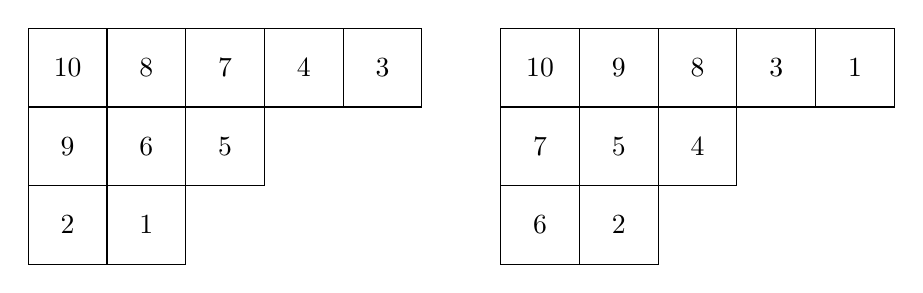
\begin{tikzpicture}

\sq{0}{0}{10}
\sq{1}{0}{8}
\sq{2}{0}{7}
\sq{3}{0}{4}
\sq{4}{0}{3}

\sq{0}{-1}{9}
\sq{1}{-1}{6}
\sq{2}{-1}{5}

\sq{0}{-2}{2}
\sq{1}{-2}{1}

\begin{scope}[xshift=6cm]

\sq{0}{0}{10}
\sq{1}{0}{9}
\sq{2}{0}{8}
\sq{3}{0}{3}
\sq{4}{0}{1}

\sq{0}{-1}{7}
\sq{1}{-1}{5}
\sq{2}{-1}{4}

\sq{0}{-2}{6}
\sq{1}{-2}{2}
\end{scope}

\end{tikzpicture}
the Robinson Schensted correspondence is a way of taking permutations and turning them into pairs of shapes like this.  And the miracle is there are exactly $n!$ as can be bound by playing \textbf{jeu de taquin}. \\ \\
And now we ask the obvious question, how do we play jeu de taquin with $\frac{1}{2} \times \frac{1}{2}$ square?

\newpage

\noindent Interesting - badly divergent infinite products - can arise in supersymmetric localization computations in theoretical physics.  Even if you don't know what that term means you can appreciate the strange number it produces:

$$  \prod_\alpha \prod_{\ell=1}^\infty \big( (\ell+1)^2 + \alpha(\sigma_0)^2\big)^{2\ell(\ell+2)}$$
Again I am not beginning to ask why or how these occur.  These are determinant of Laplacian.  Here is a matrix:
$$ \det \left[ 
\begin{array}{ccc}
1 & 0 & 0 \\ 0 & 2 & 0 \\ 0 & 0 & c
\end{array}
\right]  = 1 \times 2 \times  3 = 6$$
and you multiply all the numbers of the diagonal.  And somehow we compute 
$$ \det \nabla = \det \big( \frac{\partial^2}{\partial x^2}  +  \frac{\partial^2}{\partial y^2} \big) = \prod_{n=1}^\infty \dots $$
and the question is how we can replace $\Delta$ by an appropriate large matrix.  In the case of a sphere $$ S^3 = \{ x^2 + y^2 + z^2 + w^2 = 1\}$$
we can find a convincing basis using \textbf{spherical harmonics}.  Even the basic case:
$$ \frac{df}{dx} \approx \frac{f(x+1)- f(x-1)}{2} $$
leads to a matrix which can be diagonalized.  Or what about the less symmetric definition:
$$ \frac{df}{dx} \approx f(x+1)- f(x) $$
Or what if we incorporate scale.  Then maybe we can get appropriate answer:
$$ \frac{df}{dx} \approx \frac{f(x + \Delta x) - f(x)}{\Delta x} $$
and we have many other choices we can make which are more or less the same, but could give wildly different answers in important situations!
$$ \prod_{n=1}^\infty n^4 \stackrel{?}{=}
\big(  \prod_{n=1}^\infty n \big)^4$$
if you like just multiply all the numbers and take fourth powers.  the tradtional rules of arithmetic break down.
$$ (1 \times 2 \times 3\times 4)^4 \approx 
1^4 \times 2^4 \times 3^4 \times 4^4 $$
and - if you're really cynical - even multiplication is called into question.  why are we doing this?

\newpage 

\fontfamily{qag}\selectfont \fontsize{12}{10}\selectfont


\begin{thebibliography}{}

\item Mirjana Vuletic \textbf{A generalization of MacMahon's formula} \texttt{arXiv:0707.0532}

\item Paul Zinn-Justin \textbf{Six-Vertex, Loop and Tiling models: Integrability and Combinatorics} \texttt{arXiv:0901.0665}

\item Anton Kapustin, Brian Willett, Itamar Yaakov \textbf{Exact Results for Wilson Loops in Superconformal Chern-Simons Theories with Matter} \texttt{arXiv:0909.4559}


\end{thebibliography}



\end{document}